\section{Auswertung}
\label{sec:Auswertung}
\subsection{Berechnung der Vertikalkomponente des Erdmagnetfeldes}
Mithilfe des abgelesenen Spulenstroms der Vertikalfeldspule, welcher benötigt wurde, um die Vertikalkomponente des Erdmagnetfelds bestmöglich zu kompensieren, lässt sich diese bestimmen.\\
Abgelesen wurde am Potentiometer ein Strom von $I=\SI{0.231}{\ampere}$.\\
Nach der Versuchsanleitung \cite{Anleitung} haben die Spulen der Vertikalfeldspule jeweils einen Radius von $R=\SI{11.735}{\centi\meter}$ und eine Windungszahl von $N=20$.\\
Mit der Formel zur Berechnung des B-Felds eines Helmholtz-Spulenpaars \cite{demtröder};
\begin{equation}
\label{eqn:hholtz}
B=\mu_{\mathrm{0}} \cdot \frac{8\cdot I \cdot N}{\sqrt{125}\cdot R}
\end{equation}
ergibt sich somit für die Vertikalkomponente des Erdmagnetfelds $B_{\mathrm{vertical}}=\SI{35.4e-6}{\tesla}$.\\
Hierbei wurde die magnetische Feldkonstante $\mu_{0}$ der CODATA entnommen. \cite{mu_0}

\subsection{Messung der Transparenz der Dampfzelle}
Die Abbildung \ref{fig:oszi} zeigt ein typisches Oszilloskopbild der Tranzparenzmessung der Dampfzelle.
Da ohne anliegendes Feld keine Zeeman-Aufspaltung stattfindet, bildet sich für $B=0$ ein sehr deutlicher Nullpeak.
Hier wird das Licht der Rubidium-Spektrallampe nahezu vollständig in der Dampfzelle absorbiert. Zudem sind zwei weitere Minima der Transparenz zu erkennen.

Bei diesen Minima erzeugt das hochfrequente Wechselfeld (RF-Feld) gerade genau elektromagnetische Wellen, welche die passende Energie haben, um die vollgepumpten Niveaus zu entleeren und somit die erneute Absorption des Spektrallampenlichts in der Dampfzelle zu ermöglichen, sodass die Transparenz erneut sinkt.\\
Die notwendige Energie zum Leeren der Niveaus ist dabei abhängig von den Energiedifferenzen zwischen den Niveaus der Zeeman-Aufspaltung der Rubidium-Isotope.\\
Anhand der Tiefe der Transparenzminima soll das Verhältnis der Rubidium-Isotope in der Dampfzelle bestimmt werden.\\
Mithilfe des Pointer-Tools in der Bildbearbeitungssoftware GIMP \cite{gimp} wird anhand der Pixelposition der Minima in y-Richtung bezüglich der maximalen Transparenz das Amplitudenverhältnis der beiden Isotope bestimmt.\\
Abgelesen wird für das erste Minimum eine Tiefe von $287 \mathrm{Pixel}$ und für das zweite Minimum eine Tiefe von $496 \mathrm{Pixel}$. Es wird jeweils ein Ablesefehler von 2\% angenommen und als Unsicherheit für die weitere Berechnung mit berücksichtigt.\\
Somit ergibt sich ein Amplitudenverhältnis von
\begin{equation*}
  \frac{A_1}{A_2}=\frac{287 \pm5.8}{496 \pm 9.9}\approx 0.58\pm 0.02
\end{equation*}
\begin{figure}
  \centering
  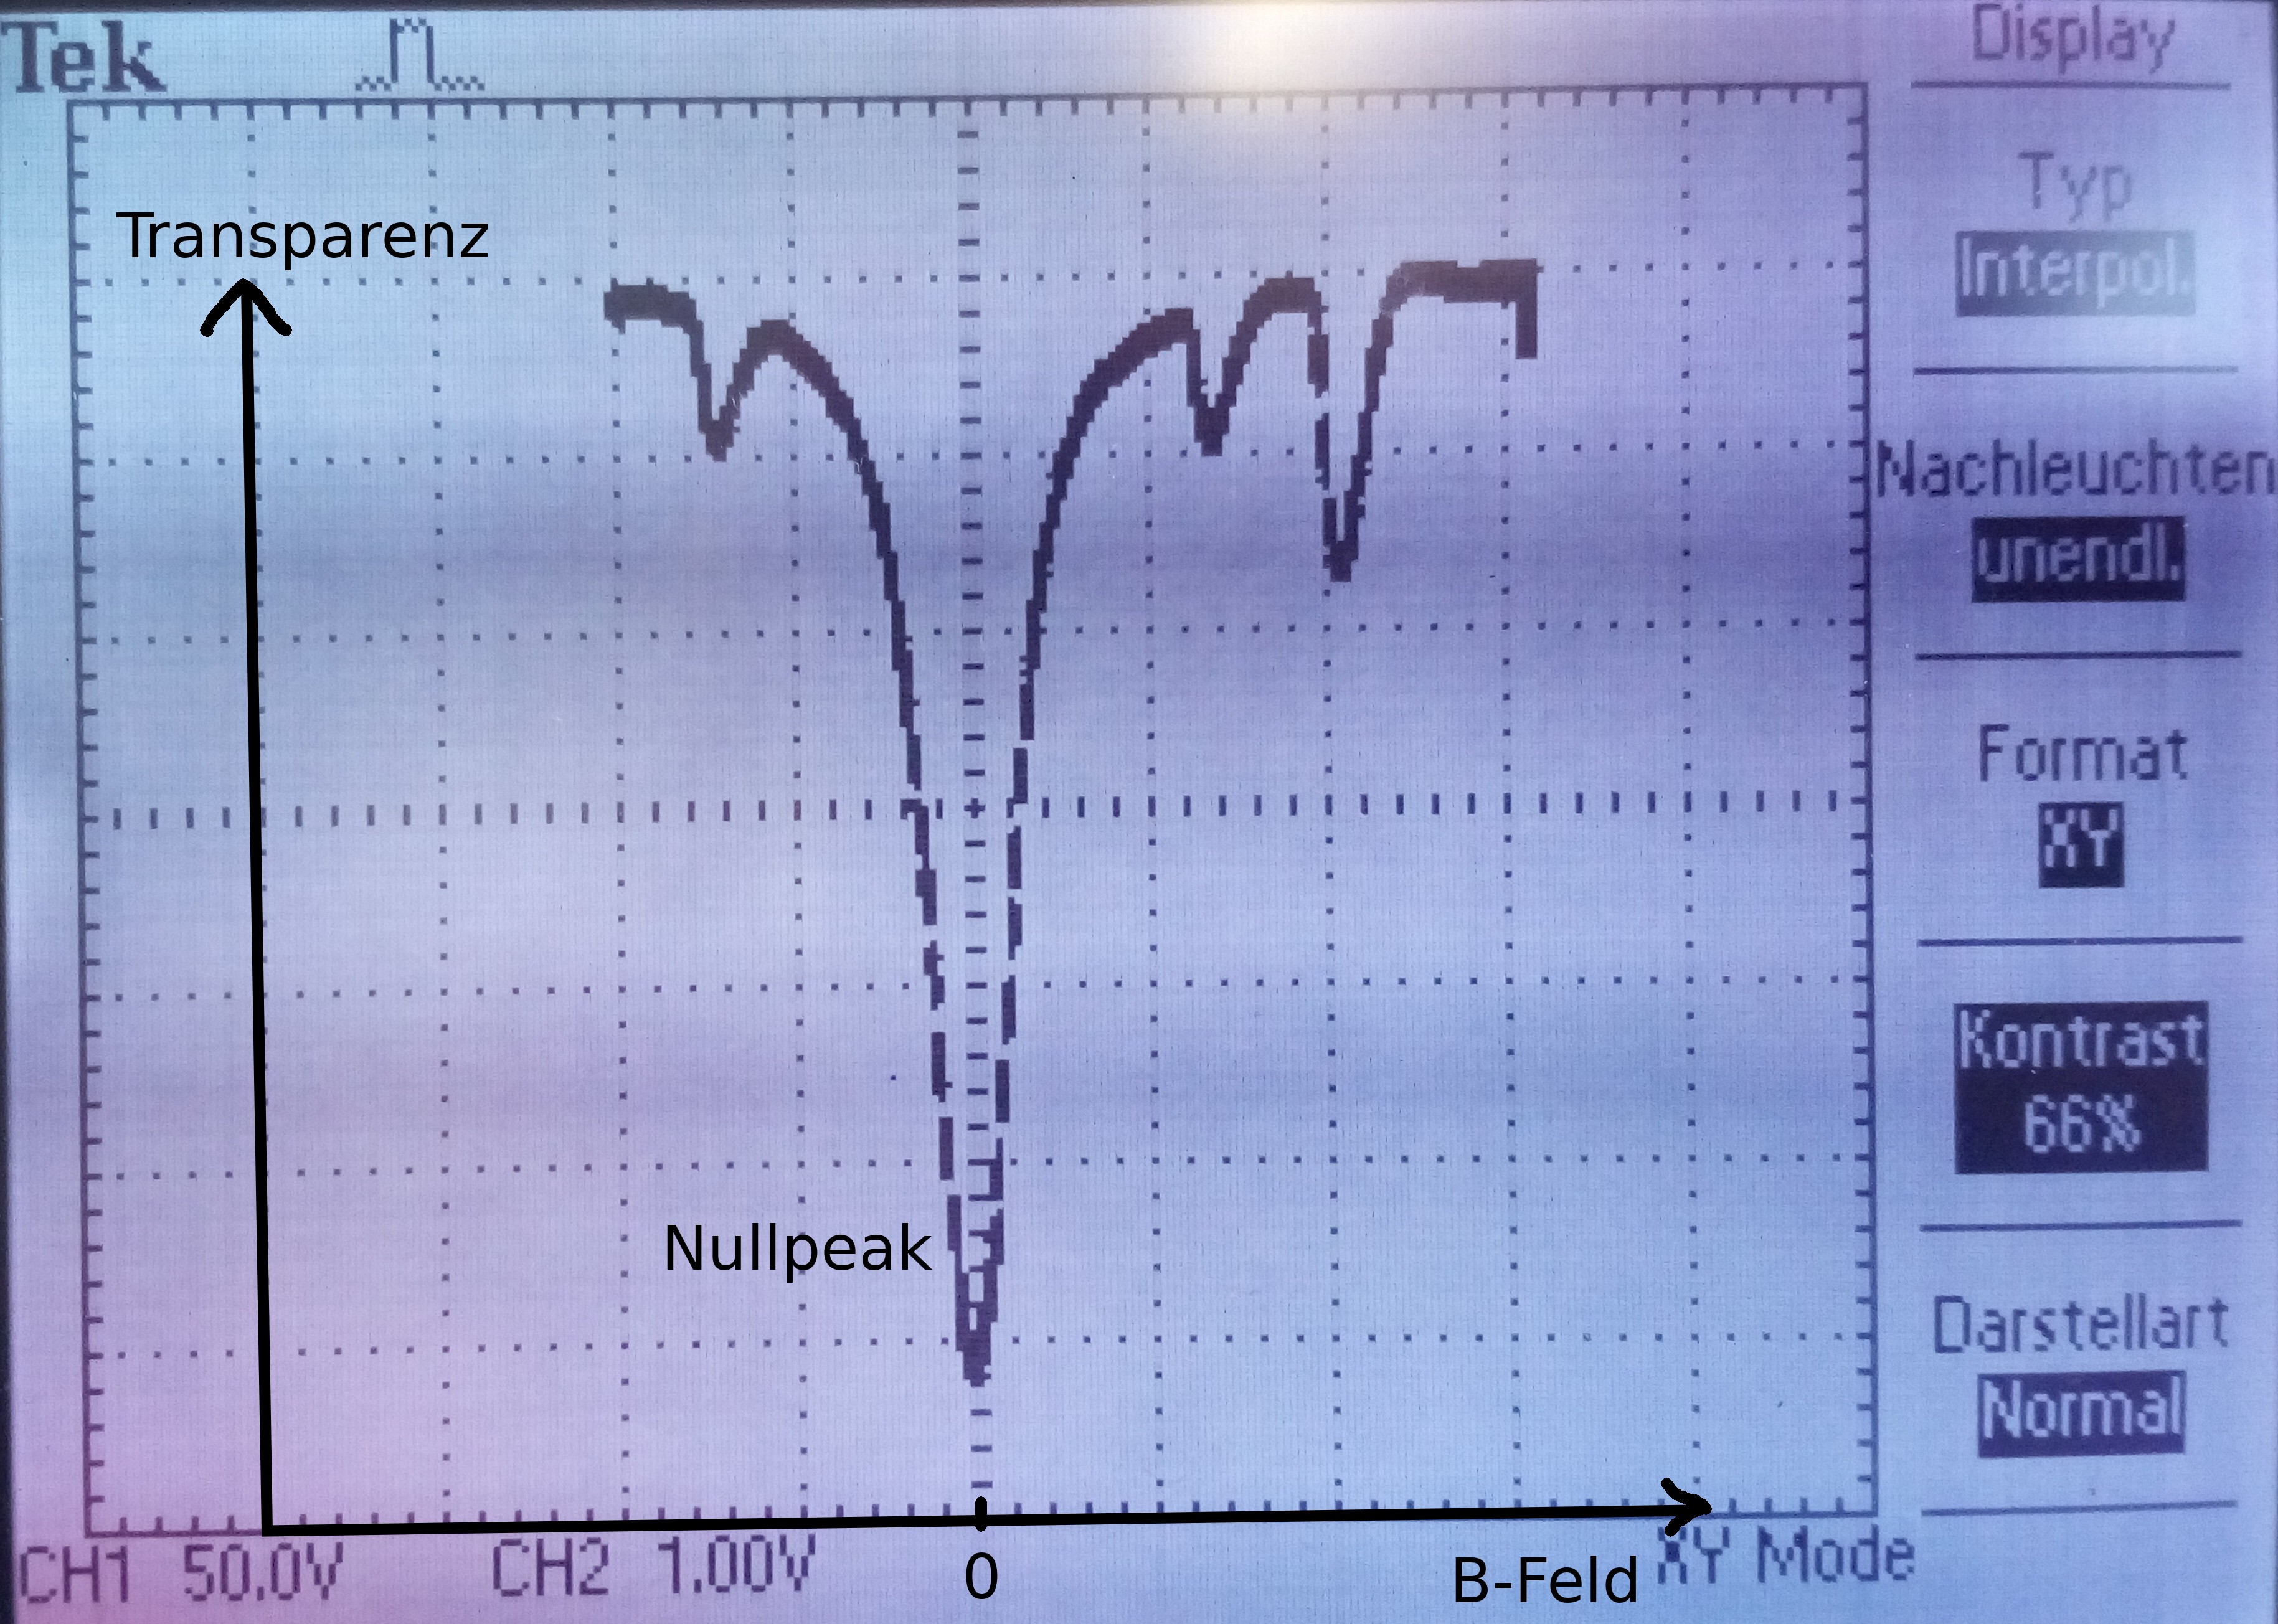
\includegraphics[width=0.9\columnwidth]{pictures/oszilloskop.jpg}
  \caption{Transparenzmessung der Dampfzelle}
  \label{fig:oszi}
\end{figure}

\subsection{Bestimmung der Horizontalkomponente des Erdmagnetfelds und der Landéschen $g_{\mathrm{F}}$-Faktoren}
Zur Bestimmung der Landé-Faktoren und der Horizontalkomponente des Erdmagnetfelds werden die Frequenzen des angelegten RF-Feldes gegen die Magnetfeldstärken in den Resonanzen der beiden Isotope aufgetragen.\\
Das gesamte B-Feld ergibt sich hierbei aus der Addition von Horizontalfeld und dem Feld der Sweep-Spule.\\
Die jeweiligen Magnetfeldstärken ergeben sich wiederum mit der Formel für die Helmholtzspule \ref{eqn:hholtz}.\\
In Tabelle \ref{tab:current} sind die gemessenen Stromstärken von Horizontalfeldspule und Sweep-Feldspule für beide Transparenzminima eingetragen.\\
Die daraus berechneten Magnetfeldstärken befinden sich ebenso in Tabelle \ref{tab:fields} wie die Frequenz des RF-Felds.\\
Das gesamte Magnetfeld, welches nötig ist um die Transparenzminima zu erzeugen, setzt sich zusammen aus dem Feld $B_{\mathrm{m}}$, welches notwendig ist, um die gepumpten Niveaus wieder zu leeren und der lokalen Horizontalkomponente des Erdmagnetfelds $B_{\mathrm{Erde}}$:
\begin{equation}
B_{\mathrm{ges}}=B_{\mathrm{m}}+B_{\mathrm{Erde}}\mathrm{.}
\end{equation}
Nach Formel \textbf{blablub} ergeben sich die $g_{\mathrm{F}}$ über die Feldstärke des RF-Felds wie folgt:
\begin{equation}
  B_{\mathrm{m}}=\frac{4\pi m_0}{e_0 g_{\mathrm{F}}}\cdot \nu \mathrm{.}
\end{equation}
Anhand obiger Überlegungen zeigt sich also ein linearer Zusammenhang zwischen dem gesamten anliegenden Magnetfeld $B_{\mathrm{ges}}$ und der Frequenz des RF-Wechselfelds:
\begin{equation}
    B_{\mathrm{ges}}=a\cdot \nu+B_{\mathrm{Erde}} \mathrm{.}
\end{equation}
In Abbildung \ref{fig:regress} sind die gemessenen gesamten B-Felder gegen die Frequenz des RF-Felds aufgetragen. Zudem wurde eine lineare Regression mittels python/scipy \cite{scipy} durchgeführt.
\begin{figure}
  \centering
  \includegraphics[width=\columnwidth]{pictures/lin_regress.pdf}
  \caption{Transparenng der Dampfzelle}
  \label{fig:regress}
\end{figure}

Die $g_{\mathrm{F}}$-Faktoren ergeben sich anschließend über den Steigungsparameter $a$ mit
\begin{equation*}
  g_{\mathrm{F}}=\frac{4\pi m_0}{e_0 a}\mathrm{.}
\end{equation*}
Die Elementarladung und die Ruhemasse des Elektron wurden der CODATA entnommen \cite{e} \cite{m_0}.
In Tabelle \ref{tab:res1} finden sich die bestimmten Regressionsparameter und die daraus berechneten Landé-Faktoren.
\begin{table}
  \caption{Regressionsparameter und Landé-Faktoren beider Isotope}
  \label{tab:res1}
 \centering
 \begin{tabular}{cccc}
   \toprule
&Steigungsparameter $a_i$ /$ 10^{-12}\si{\tesla\per\hertz}$&$g_{\mathrm{F}}$&$B_{\mathrm{Erd}}$/$10^{-6}\si{\tesla}$\\
\midrule
Isotop 1&$142.06\pm1.49$&$0.503\pm0.005$&$18.86\pm0.92$\\
Isotop2&$215.19\pm0.61$&$0.332\pm0.001$ &$17.69\pm0.38$\\
\bottomrule
\end{tabular}
\end{table}
Der Mittelwert (gebildet mittels python/numpy \cite{numpy}) der y-Achsenabschnitte der Ausgleichsgrade beider Isotope ergibt die lokale Horizontalkomponente des Erdmagnetfelds zu $B_{\mathrm{Erde,ges}}=\SI{18.3(5)e-6}{\tesla}$.

\begin{table}
 \caption{Im Experiment gemessene Ströme der Sweep-Spule und der Horizontalfeldspule für die Transparenzminima beider Isotope sowie die Frequenz des angelegten RF-Wechselfelds }
 \label{tab:current}
 \centering
 \begin{tabular}{ccccc}
 \toprule 
    RF-Wechselfeld/$\si{\kilo\hertz}$ & $I_{\mathrm{Horizontal,1}}/\si{\milli \ampere}$ & $I_{\mathrm{Horizontal,2}}/\si{\milli \ampere}$ & $I_{\mathrm{Sweep,1}}/\si{\milli \ampere}$ & $I_{\mathrm{Sweep,2}}/\si{\milli \ampere}$ \\
     \midrule
     100.3 & 0 & 0 & 597 & 666 \\
     201.0 & 35 & 35 & 245 & 484 \\
     301.0 & 56 & 56 & 187 & 545 \\
     400.0 & 76 & 76 & 139 & 617 \\
     499.0 & 91 & 91 & 162 & 753 \\
     603.0 & 116 & 116 & 47 & 763 \\
     699.0 & 88 & 159 & 688 & 473 \\
     801.0 & 101 & 182 & 736 & 508 \\
     899.0 & 149 & 207 & 265 & 493 \\
     1004.0 & 156 & 237 & 410 & 424 \\
 \bottomrule
 \end{tabular}
\end{table}
\begin{table}
 \caption{Aus den gemessenen Strömen berechnete B-Felder für die Horizontalfeldspule und die Sweep-Spule $B_{\mathrm{Swp}}$ in den Transparenzminima beider Isotope}
 \label{tab:fields}
 \centering
 \begin{tabular}{ccccc}
 \toprule 
    RF-Feld/$\si{\kilo\hertz}$ & $B_{\mathrm{Horizontal,1}}/10^{-6}\si{\tesla}$ & $B_{\mathrm{Horizontal,2}}/10^{-6}\si{\tesla}$ & $B_{\mathrm{Swp,1}}/10^{-6}\si{\tesla}$ & $B_{\mathrm{Swp,2}}/10^{-6}\si{\tesla}$ \\
     \midrule
     100.3 & 36.03 & 40.19 & 0.0 & 0.0 \\
     201.0 & 14.79 & 29.21 & 30.69 & 30.69 \\
     301.0 & 11.28 & 32.89 & 49.11 & 49.11 \\
     400.0 & 8.39 & 37.23 & 66.65 & 66.65 \\
     499.0 & 9.78 & 45.44 & 79.8 & 79.8 \\
     603.0 & 2.84 & 46.05 & 101.73 & 101.73 \\
     699.0 & 41.52 & 28.54 & 77.17 & 139.44 \\
     801.0 & 44.42 & 30.66 & 88.57 & 159.61 \\
     899.0 & 15.99 & 29.75 & 130.67 & 181.53 \\
     1004.0 & 24.74 & 25.59 & 136.81 & 207.84 \\
 \bottomrule
 \end{tabular}
\end{table}

\subsection{Bestimmung der Kernspins beider Isotope}
Das hier betrachtete Rubidium ist ein Alkalimetall und hat daher ein einzelnes Elektron auf einer s-Schale (bei Rubidium ist dies die 5s-Schale), welches den Gesamtspin der Elektronenhülle bestimmt.\\
Somit hat die Elektronenhülle keinen Drehimpuls, also $L=0$ und ihr Gesamtspin ergibt sich zu $J=S=1/2$. Da für den Gesamtspin des Atoms $F=I+J$ gilt, ergibt sich mit Formel blablup:
\begin{equation*}
I=\frac{g_{\mathrm{J}}}{2\cdot g_{\mathrm{F}}}-\frac{1}{2}
\end{equation*}
Es ist $g_{\mathrm{J}}=g_{\mathrm{S}}=2.00232$ nach Versuchsanleitung \cite{Anleitung}.
Für die beiden Isotope ergibt sich:
\begin{gather*}
  I_{\mathrm{Isotop 1}}=1.491\pm0.021\approx\frac{3}{2}\\
  I_{\mathrm{Isotop 2}}=2.515\pm0.009\approx\frac{5}{2}\\
\end{gather*}

Da der Kernspin nur Vielfache von $\frac{1}{2}$ annimmt, wurde jeweils auf das nächste Vielfache gerundet.\\
Ein Vergleich mit der Literaturwerten der Kernspins zeigt, dass es sich bei $I_{\mathrm{Isotop 1}}$ um $\ce{^87Rb}$ und bei $I_{\mathrm{Isotop 2}}$ höchstwahrscheinlich um $\ce{^85Rb}$ handelt \cite{muenster}.

\subsection{Quadratischer Zeeman-Effekt}
Der quadratische Zeeman-Effekt spielt nur für große Magnetfelder eine Rolle. \\
Im Folgenden wird dieser anhand der hier verwendeten Rubidium-Isotope und den genutzten Magnetfeldern abgeschätzt.
Mit $M_{\mathrm{J}}=0$, \Delta$E_{\mathrm{Hy}}\approx\SI{1e-24}{\joule}$ \cite{Anleitung}, $g_{\mathrm{F}}\approx 0.5$ und Magnetfeldern von maximal $B=\SI{250e-6}{\tesla}$ würden sich über den quadratischen Zeeman-Effekt nach Formel blablabla ein Korrekturterm der Übergangsenergie $U_{\mathrm{HF}}$ in der Größenordnung $U_{\mathrm{HF}}\approx \SI{1e-31}{\joule}$ ergeben.\\
Der normale Zeeman-Effekt ist etwa in der Größenordnung $U_{\mathrm{HF}}\approx \SI{1e-27}{\joule}$ und damit vier Größenordnungen größer. Daher spielt der quadratische Zeeman-Effekt im vorliegenden Experiment keine Rolle.
